\documentclass[twoside]{book}

% Packages required by doxygen
\usepackage{calc}
\usepackage{doxygen}
\usepackage{graphicx}
\usepackage[utf8]{inputenc}
\usepackage{makeidx}
\usepackage{multicol}
\usepackage{multirow}
\usepackage{textcomp}
\usepackage[table]{xcolor}

% Font selection
\usepackage[T1]{fontenc}
\usepackage{mathptmx}
\usepackage[scaled=.90]{helvet}
\usepackage{courier}
\usepackage{amssymb}
\usepackage{sectsty}
\renewcommand{\familydefault}{\sfdefault}
\allsectionsfont{%
  \fontseries{bc}\selectfont%
  \color{darkgray}%
}
\renewcommand{\DoxyLabelFont}{%
  \fontseries{bc}\selectfont%
  \color{darkgray}%
}

% Page & text layout
\usepackage{geometry}
\geometry{%
  a4paper,%
  top=2.5cm,%
  bottom=2.5cm,%
  left=2.5cm,%
  right=2.5cm%
}
\tolerance=750
\hfuzz=15pt
\hbadness=750
\setlength{\emergencystretch}{15pt}
\setlength{\parindent}{0cm}
\setlength{\parskip}{0.2cm}
\makeatletter
\renewcommand{\paragraph}{%
  \@startsection{paragraph}{4}{0ex}{-1.0ex}{1.0ex}{%
    \normalfont\normalsize\bfseries\SS@parafont%
  }%
}
\renewcommand{\subparagraph}{%
  \@startsection{subparagraph}{5}{0ex}{-1.0ex}{1.0ex}{%
    \normalfont\normalsize\bfseries\SS@subparafont%
  }%
}
\makeatother

% Headers & footers
\usepackage{fancyhdr}
\pagestyle{fancyplain}
\fancyhead[LE]{\fancyplain{}{\bfseries\thepage}}
\fancyhead[CE]{\fancyplain{}{}}
\fancyhead[RE]{\fancyplain{}{\bfseries\leftmark}}
\fancyhead[LO]{\fancyplain{}{\bfseries\rightmark}}
\fancyhead[CO]{\fancyplain{}{}}
\fancyhead[RO]{\fancyplain{}{\bfseries\thepage}}
\fancyfoot[LE]{\fancyplain{}{}}
\fancyfoot[CE]{\fancyplain{}{}}
\fancyfoot[RE]{\fancyplain{}{\bfseries\scriptsize Generated on Fri Jun 13 2014 12\-:28\-:40 for Ph2\-\_\-\-Hw\-Interface by Doxygen }}
\fancyfoot[LO]{\fancyplain{}{\bfseries\scriptsize Generated on Fri Jun 13 2014 12\-:28\-:40 for Ph2\-\_\-\-Hw\-Interface by Doxygen }}
\fancyfoot[CO]{\fancyplain{}{}}
\fancyfoot[RO]{\fancyplain{}{}}
\renewcommand{\footrulewidth}{0.4pt}
\renewcommand{\chaptermark}[1]{%
  \markboth{#1}{}%
}
\renewcommand{\sectionmark}[1]{%
  \markright{\thesection\ #1}%
}

% Indices & bibliography
\usepackage{natbib}
\usepackage[titles]{tocloft}
\setcounter{tocdepth}{3}
\setcounter{secnumdepth}{5}
\makeindex

% Hyperlinks (required, but should be loaded last)
\usepackage{ifpdf}
\ifpdf
  \usepackage[pdftex,pagebackref=true]{hyperref}
\else
  \usepackage[ps2pdf,pagebackref=true]{hyperref}
\fi
\hypersetup{%
  colorlinks=true,%
  linkcolor=blue,%
  citecolor=blue,%
  unicode%
}

% Custom commands
\newcommand{\clearemptydoublepage}{%
  \newpage{\pagestyle{empty}\cleardoublepage}%
}


%===== C O N T E N T S =====

\begin{document}

% Titlepage & ToC
\hypersetup{pageanchor=false}
\pagenumbering{roman}
\begin{titlepage}
\vspace*{7cm}
\begin{center}%
{\Large Ph2\-\_\-\-Hw\-Interface \\[1ex]\large 1.\-1 }\\
\vspace*{1cm}
{\large Generated by Doxygen 1.8.5}\\
\vspace*{0.5cm}
{\small Fri Jun 13 2014 12:28:40}\\
\end{center}
\end{titlepage}
\clearemptydoublepage
\tableofcontents
\clearemptydoublepage
\pagenumbering{arabic}
\hypersetup{pageanchor=true}

%--- Begin generated contents ---
\chapter{Hierarchical Index}
\section{Class Hierarchy}
This inheritance list is sorted roughly, but not completely, alphabetically\-:\begin{DoxyCompactList}
\item \contentsline{section}{Ph2\-\_\-\-Hw\-Description\-:\-:Be\-Board}{\pageref{class_ph2___hw_description_1_1_be_board}}{}
\begin{DoxyCompactList}
\item \contentsline{section}{Ph2\-\_\-\-Hw\-Description\-:\-:Glib}{\pageref{class_ph2___hw_description_1_1_glib}}{}
\end{DoxyCompactList}
\item \contentsline{section}{Ph2\-\_\-\-Hw\-Description\-:\-:Cbc\-Comparer}{\pageref{struct_ph2___hw_description_1_1_cbc_comparer}}{}
\item \contentsline{section}{Ph2\-\_\-\-Hw\-Description\-:\-:Cbc\-Reg\-Item}{\pageref{struct_ph2___hw_description_1_1_cbc_reg_item}}{}
\item \contentsline{section}{Ph2\-\_\-\-Hw\-Interface\-:\-:Data}{\pageref{class_ph2___hw_interface_1_1_data}}{}
\item \contentsline{section}{Ph2\-\_\-\-Hw\-Interface\-:\-:Event}{\pageref{class_ph2___hw_interface_1_1_event}}{}
\item exception\begin{DoxyCompactList}
\item \contentsline{section}{Ph2\-\_\-\-Hw\-Interface\-:\-:Exception}{\pageref{class_ph2___hw_interface_1_1_exception}}{}
\end{DoxyCompactList}
\item \contentsline{section}{Ph2\-\_\-\-Hw\-Description\-:\-:Front\-End\-Description}{\pageref{class_ph2___hw_description_1_1_front_end_description}}{}
\begin{DoxyCompactList}
\item \contentsline{section}{Ph2\-\_\-\-Hw\-Description\-:\-:Cbc}{\pageref{class_ph2___hw_description_1_1_cbc}}{}
\item \contentsline{section}{Ph2\-\_\-\-Hw\-Description\-:\-:Module}{\pageref{class_ph2___hw_description_1_1_module}}{}
\end{DoxyCompactList}
\item \contentsline{section}{Ph2\-\_\-\-Hw\-Interface\-:\-:Reg\-Manager}{\pageref{class_ph2___hw_interface_1_1_reg_manager}}{}
\begin{DoxyCompactList}
\item \contentsline{section}{Ph2\-\_\-\-Hw\-Interface\-:\-:Be\-Board\-Interface}{\pageref{class_ph2___hw_interface_1_1_be_board_interface}}{}
\item \contentsline{section}{Ph2\-\_\-\-Hw\-Interface\-:\-:Cbc\-Interface}{\pageref{class_ph2___hw_interface_1_1_cbc_interface}}{}
\item \contentsline{section}{Ph2\-\_\-\-Hw\-Interface\-:\-:Glib\-Interface}{\pageref{class_ph2___hw_interface_1_1_glib_interface}}{}
\end{DoxyCompactList}
\end{DoxyCompactList}

\chapter{Data Structure Index}
\section{Class List}
Here are the classes, structs, unions and interfaces with brief descriptions\-:\begin{DoxyCompactList}
\item\contentsline{section}{\hyperlink{class_interface_1_1_h_w_interface}{Interface\-::\-H\-W\-Interface} }{\pageref{class_interface_1_1_h_w_interface}}{}
\end{DoxyCompactList}

\chapter{Data Structure Documentation}
\hypertarget{class_ph2___hw_interface_1_1_c_b_c_interface}{\section{Ph2\-\_\-\-Hw\-Interface\-:\-:C\-B\-C\-Interface Class Reference}
\label{class_ph2___hw_interface_1_1_c_b_c_interface}\index{Ph2\-\_\-\-Hw\-Interface\-::\-C\-B\-C\-Interface@{Ph2\-\_\-\-Hw\-Interface\-::\-C\-B\-C\-Interface}}
}


{\ttfamily \#include $<$Cbc\-Interface.\-h$>$}

Inheritance diagram for Ph2\-\_\-\-Hw\-Interface\-:\-:C\-B\-C\-Interface\-:\begin{figure}[H]
\begin{center}
\leavevmode
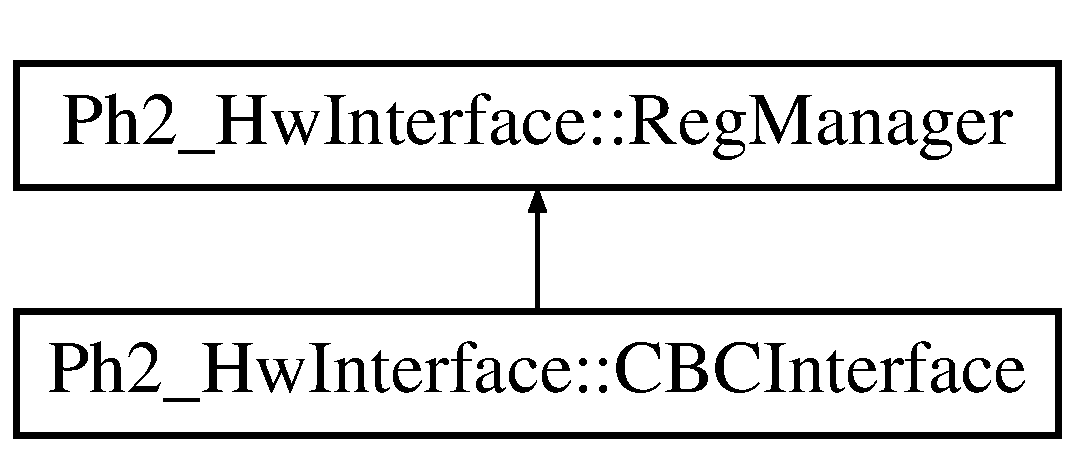
\includegraphics[height=2.000000cm]{class_ph2___hw_interface_1_1_c_b_c_interface}
\end{center}
\end{figure}
\subsection*{Public Member Functions}
\begin{DoxyCompactItemize}
\item 
\hyperlink{class_ph2___hw_interface_1_1_c_b_c_interface_ac6d2dce57f278cc0678c32ae432187e4}{C\-B\-C\-Interface} ()
\item 
\hyperlink{class_ph2___hw_interface_1_1_c_b_c_interface_a28d0a36d433bae296ff3980c80b3b1cd}{$\sim$\-C\-B\-C\-Interface} ()
\item 
void \hyperlink{class_ph2___hw_interface_1_1_c_b_c_interface_aecf7769a1863999fd05efca3993d3b92}{Select\-Sram\-For\-I2\-C} (unsigned int p\-Fe)
\item 
bool \hyperlink{class_ph2___hw_interface_1_1_c_b_c_interface_a8dff31d5f9575070179612b5b9335aa4}{I2c\-Cmd\-Ack\-Wait} (uint32\-\_\-t p\-Ack\-Val, unsigned int p\-Ncount=1)
\item 
void \hyperlink{class_ph2___hw_interface_1_1_c_b_c_interface_af6eeb7700b550a51acca3441180ddc33}{Send\-Block\-Cbc\-I2c\-Request} (uint32\-\_\-t p\-Fe, std\-::vector$<$ uint32\-\_\-t $>$ \&p\-Vec\-Req, bool p\-Write)
\item 
void \hyperlink{class_ph2___hw_interface_1_1_c_b_c_interface_a07b718e617fb6e992764c724edd4d406}{Read\-I2c\-Values\-In\-S\-R\-A\-M} (unsigned int p\-Fe, std\-::vector$<$ uint32\-\_\-t $>$ \&p\-Vec\-Req)
\item 
void \hyperlink{class_ph2___hw_interface_1_1_c_b_c_interface_ad79c9b9ec21e78d35fd0c62e48ba6784}{Enable\-I2c} (bool p\-Enable)
\item 
uint32\-\_\-t \hyperlink{class_ph2___hw_interface_1_1_c_b_c_interface_a9c34bda282edef6fec34245969ac59a0}{Send\-I2c} (uint16\-\_\-t p\-Addr, uint16\-\_\-t p\-Data, bool p\-Write)
\end{DoxyCompactItemize}
\subsection*{Static Public Attributes}
\begin{DoxyCompactItemize}
\item 
static const std\-::string \hyperlink{class_ph2___hw_interface_1_1_c_b_c_interface_a3e1a76026b451e23697eb1eecdf8c912}{f\-Str\-I2c\-Settings} = \hyperlink{_cbc_interface_8cc_a15db09e24617ea5c5843213672ac8a03}{I2\-C\-\_\-\-S\-E\-T\-T\-I\-N\-G\-S}
\item 
static const std\-::string \hyperlink{class_ph2___hw_interface_1_1_c_b_c_interface_a2c72e9920d45e1df938f582a095196d4}{f\-Str\-I2c\-Command} = \hyperlink{_cbc_interface_8cc_ae308275dafb538f2511ea285fea768d0}{I2\-C\-\_\-\-C\-O\-M\-M\-A\-N\-D}
\item 
static const std\-::string \hyperlink{class_ph2___hw_interface_1_1_c_b_c_interface_a583ceda969e6d70c981cad62af51f567}{f\-Str\-I2c\-Reply} = \hyperlink{_cbc_interface_8cc_a46aaa2293185dfc3cd655f65bea7f614}{I2\-C\-\_\-\-R\-E\-P\-L\-Y}
\item 
static const uint32\-\_\-t \hyperlink{class_ph2___hw_interface_1_1_c_b_c_interface_a5222dcc6e69a64dcef874d622136e994}{f\-I2c\-Slave} = \hyperlink{_cbc_interface_8cc_ab15137f7c592d05573de99f078516157}{I2\-C\-\_\-\-S\-L\-A\-V\-E}
\end{DoxyCompactItemize}
\subsection*{Private Attributes}
\begin{DoxyCompactItemize}
\item 
std\-::string \hyperlink{class_ph2___hw_interface_1_1_c_b_c_interface_a19496098840524d937006e847a82ab37}{f\-Str\-Sram}
\item 
std\-::string \hyperlink{class_ph2___hw_interface_1_1_c_b_c_interface_a23c250eabca85a5cb7042dca0f3be50c}{f\-Str\-Other\-Sram}
\item 
std\-::string \hyperlink{class_ph2___hw_interface_1_1_c_b_c_interface_ac74f8185e2194b9697833c5307d031ea}{f\-Str\-Sram\-User\-Logic}
\item 
std\-::string \hyperlink{class_ph2___hw_interface_1_1_c_b_c_interface_ad7cefdc3aade4b4ddc9d63fee1f09b1e}{f\-Str\-Full}
\item 
std\-::string \hyperlink{class_ph2___hw_interface_1_1_c_b_c_interface_a1f52dd280bb04707d890526be58b56ba}{f\-Str\-Readout}
\end{DoxyCompactItemize}
\subsection*{Additional Inherited Members}


\subsection{Constructor \& Destructor Documentation}
\hypertarget{class_ph2___hw_interface_1_1_c_b_c_interface_ac6d2dce57f278cc0678c32ae432187e4}{\index{Ph2\-\_\-\-Hw\-Interface\-::\-C\-B\-C\-Interface@{Ph2\-\_\-\-Hw\-Interface\-::\-C\-B\-C\-Interface}!C\-B\-C\-Interface@{C\-B\-C\-Interface}}
\index{C\-B\-C\-Interface@{C\-B\-C\-Interface}!Ph2_HwInterface::CBCInterface@{Ph2\-\_\-\-Hw\-Interface\-::\-C\-B\-C\-Interface}}
\subsubsection[{C\-B\-C\-Interface}]{\setlength{\rightskip}{0pt plus 5cm}Ph2\-\_\-\-Hw\-Interface\-::\-C\-B\-C\-Interface\-::\-C\-B\-C\-Interface (
\begin{DoxyParamCaption}
{}
\end{DoxyParamCaption}
)}}\label{class_ph2___hw_interface_1_1_c_b_c_interface_ac6d2dce57f278cc0678c32ae432187e4}
\hypertarget{class_ph2___hw_interface_1_1_c_b_c_interface_a28d0a36d433bae296ff3980c80b3b1cd}{\index{Ph2\-\_\-\-Hw\-Interface\-::\-C\-B\-C\-Interface@{Ph2\-\_\-\-Hw\-Interface\-::\-C\-B\-C\-Interface}!$\sim$\-C\-B\-C\-Interface@{$\sim$\-C\-B\-C\-Interface}}
\index{$\sim$\-C\-B\-C\-Interface@{$\sim$\-C\-B\-C\-Interface}!Ph2_HwInterface::CBCInterface@{Ph2\-\_\-\-Hw\-Interface\-::\-C\-B\-C\-Interface}}
\subsubsection[{$\sim$\-C\-B\-C\-Interface}]{\setlength{\rightskip}{0pt plus 5cm}Ph2\-\_\-\-Hw\-Interface\-::\-C\-B\-C\-Interface\-::$\sim$\-C\-B\-C\-Interface (
\begin{DoxyParamCaption}
{}
\end{DoxyParamCaption}
)}}\label{class_ph2___hw_interface_1_1_c_b_c_interface_a28d0a36d433bae296ff3980c80b3b1cd}


\subsection{Member Function Documentation}
\hypertarget{class_ph2___hw_interface_1_1_c_b_c_interface_ad79c9b9ec21e78d35fd0c62e48ba6784}{\index{Ph2\-\_\-\-Hw\-Interface\-::\-C\-B\-C\-Interface@{Ph2\-\_\-\-Hw\-Interface\-::\-C\-B\-C\-Interface}!Enable\-I2c@{Enable\-I2c}}
\index{Enable\-I2c@{Enable\-I2c}!Ph2_HwInterface::CBCInterface@{Ph2\-\_\-\-Hw\-Interface\-::\-C\-B\-C\-Interface}}
\subsubsection[{Enable\-I2c}]{\setlength{\rightskip}{0pt plus 5cm}void Ph2\-\_\-\-Hw\-Interface\-::\-C\-B\-C\-Interface\-::\-Enable\-I2c (
\begin{DoxyParamCaption}
\item[{bool}]{p\-Enable}
\end{DoxyParamCaption}
)}}\label{class_ph2___hw_interface_1_1_c_b_c_interface_ad79c9b9ec21e78d35fd0c62e48ba6784}
\hypertarget{class_ph2___hw_interface_1_1_c_b_c_interface_a8dff31d5f9575070179612b5b9335aa4}{\index{Ph2\-\_\-\-Hw\-Interface\-::\-C\-B\-C\-Interface@{Ph2\-\_\-\-Hw\-Interface\-::\-C\-B\-C\-Interface}!I2c\-Cmd\-Ack\-Wait@{I2c\-Cmd\-Ack\-Wait}}
\index{I2c\-Cmd\-Ack\-Wait@{I2c\-Cmd\-Ack\-Wait}!Ph2_HwInterface::CBCInterface@{Ph2\-\_\-\-Hw\-Interface\-::\-C\-B\-C\-Interface}}
\subsubsection[{I2c\-Cmd\-Ack\-Wait}]{\setlength{\rightskip}{0pt plus 5cm}bool Ph2\-\_\-\-Hw\-Interface\-::\-C\-B\-C\-Interface\-::\-I2c\-Cmd\-Ack\-Wait (
\begin{DoxyParamCaption}
\item[{uint32\-\_\-t}]{p\-Ack\-Val, }
\item[{unsigned int}]{p\-Ncount = {\ttfamily 1}}
\end{DoxyParamCaption}
)}}\label{class_ph2___hw_interface_1_1_c_b_c_interface_a8dff31d5f9575070179612b5b9335aa4}
\hypertarget{class_ph2___hw_interface_1_1_c_b_c_interface_a07b718e617fb6e992764c724edd4d406}{\index{Ph2\-\_\-\-Hw\-Interface\-::\-C\-B\-C\-Interface@{Ph2\-\_\-\-Hw\-Interface\-::\-C\-B\-C\-Interface}!Read\-I2c\-Values\-In\-S\-R\-A\-M@{Read\-I2c\-Values\-In\-S\-R\-A\-M}}
\index{Read\-I2c\-Values\-In\-S\-R\-A\-M@{Read\-I2c\-Values\-In\-S\-R\-A\-M}!Ph2_HwInterface::CBCInterface@{Ph2\-\_\-\-Hw\-Interface\-::\-C\-B\-C\-Interface}}
\subsubsection[{Read\-I2c\-Values\-In\-S\-R\-A\-M}]{\setlength{\rightskip}{0pt plus 5cm}void Ph2\-\_\-\-Hw\-Interface\-::\-C\-B\-C\-Interface\-::\-Read\-I2c\-Values\-In\-S\-R\-A\-M (
\begin{DoxyParamCaption}
\item[{unsigned int}]{p\-Fe, }
\item[{std\-::vector$<$ uint32\-\_\-t $>$ \&}]{p\-Vec\-Req}
\end{DoxyParamCaption}
)}}\label{class_ph2___hw_interface_1_1_c_b_c_interface_a07b718e617fb6e992764c724edd4d406}
\hypertarget{class_ph2___hw_interface_1_1_c_b_c_interface_aecf7769a1863999fd05efca3993d3b92}{\index{Ph2\-\_\-\-Hw\-Interface\-::\-C\-B\-C\-Interface@{Ph2\-\_\-\-Hw\-Interface\-::\-C\-B\-C\-Interface}!Select\-Sram\-For\-I2\-C@{Select\-Sram\-For\-I2\-C}}
\index{Select\-Sram\-For\-I2\-C@{Select\-Sram\-For\-I2\-C}!Ph2_HwInterface::CBCInterface@{Ph2\-\_\-\-Hw\-Interface\-::\-C\-B\-C\-Interface}}
\subsubsection[{Select\-Sram\-For\-I2\-C}]{\setlength{\rightskip}{0pt plus 5cm}void Ph2\-\_\-\-Hw\-Interface\-::\-C\-B\-C\-Interface\-::\-Select\-Sram\-For\-I2\-C (
\begin{DoxyParamCaption}
\item[{unsigned int}]{p\-Fe}
\end{DoxyParamCaption}
)}}\label{class_ph2___hw_interface_1_1_c_b_c_interface_aecf7769a1863999fd05efca3993d3b92}
\hypertarget{class_ph2___hw_interface_1_1_c_b_c_interface_af6eeb7700b550a51acca3441180ddc33}{\index{Ph2\-\_\-\-Hw\-Interface\-::\-C\-B\-C\-Interface@{Ph2\-\_\-\-Hw\-Interface\-::\-C\-B\-C\-Interface}!Send\-Block\-Cbc\-I2c\-Request@{Send\-Block\-Cbc\-I2c\-Request}}
\index{Send\-Block\-Cbc\-I2c\-Request@{Send\-Block\-Cbc\-I2c\-Request}!Ph2_HwInterface::CBCInterface@{Ph2\-\_\-\-Hw\-Interface\-::\-C\-B\-C\-Interface}}
\subsubsection[{Send\-Block\-Cbc\-I2c\-Request}]{\setlength{\rightskip}{0pt plus 5cm}void Ph2\-\_\-\-Hw\-Interface\-::\-C\-B\-C\-Interface\-::\-Send\-Block\-Cbc\-I2c\-Request (
\begin{DoxyParamCaption}
\item[{uint32\-\_\-t}]{p\-Fe, }
\item[{std\-::vector$<$ uint32\-\_\-t $>$ \&}]{p\-Vec\-Req, }
\item[{bool}]{p\-Write}
\end{DoxyParamCaption}
)}}\label{class_ph2___hw_interface_1_1_c_b_c_interface_af6eeb7700b550a51acca3441180ddc33}
\hypertarget{class_ph2___hw_interface_1_1_c_b_c_interface_a9c34bda282edef6fec34245969ac59a0}{\index{Ph2\-\_\-\-Hw\-Interface\-::\-C\-B\-C\-Interface@{Ph2\-\_\-\-Hw\-Interface\-::\-C\-B\-C\-Interface}!Send\-I2c@{Send\-I2c}}
\index{Send\-I2c@{Send\-I2c}!Ph2_HwInterface::CBCInterface@{Ph2\-\_\-\-Hw\-Interface\-::\-C\-B\-C\-Interface}}
\subsubsection[{Send\-I2c}]{\setlength{\rightskip}{0pt plus 5cm}uint32\-\_\-t Ph2\-\_\-\-Hw\-Interface\-::\-C\-B\-C\-Interface\-::\-Send\-I2c (
\begin{DoxyParamCaption}
\item[{uint16\-\_\-t}]{p\-Addr, }
\item[{uint16\-\_\-t}]{p\-Data, }
\item[{bool}]{p\-Write}
\end{DoxyParamCaption}
)}}\label{class_ph2___hw_interface_1_1_c_b_c_interface_a9c34bda282edef6fec34245969ac59a0}


\subsection{Field Documentation}
\hypertarget{class_ph2___hw_interface_1_1_c_b_c_interface_a5222dcc6e69a64dcef874d622136e994}{\index{Ph2\-\_\-\-Hw\-Interface\-::\-C\-B\-C\-Interface@{Ph2\-\_\-\-Hw\-Interface\-::\-C\-B\-C\-Interface}!f\-I2c\-Slave@{f\-I2c\-Slave}}
\index{f\-I2c\-Slave@{f\-I2c\-Slave}!Ph2_HwInterface::CBCInterface@{Ph2\-\_\-\-Hw\-Interface\-::\-C\-B\-C\-Interface}}
\subsubsection[{f\-I2c\-Slave}]{\setlength{\rightskip}{0pt plus 5cm}const uint32\-\_\-t Ph2\-\_\-\-Hw\-Interface\-::\-C\-B\-C\-Interface\-::f\-I2c\-Slave = {\bf I2\-C\-\_\-\-S\-L\-A\-V\-E}\hspace{0.3cm}{\ttfamily [static]}}}\label{class_ph2___hw_interface_1_1_c_b_c_interface_a5222dcc6e69a64dcef874d622136e994}
\hypertarget{class_ph2___hw_interface_1_1_c_b_c_interface_ad7cefdc3aade4b4ddc9d63fee1f09b1e}{\index{Ph2\-\_\-\-Hw\-Interface\-::\-C\-B\-C\-Interface@{Ph2\-\_\-\-Hw\-Interface\-::\-C\-B\-C\-Interface}!f\-Str\-Full@{f\-Str\-Full}}
\index{f\-Str\-Full@{f\-Str\-Full}!Ph2_HwInterface::CBCInterface@{Ph2\-\_\-\-Hw\-Interface\-::\-C\-B\-C\-Interface}}
\subsubsection[{f\-Str\-Full}]{\setlength{\rightskip}{0pt plus 5cm}std\-::string Ph2\-\_\-\-Hw\-Interface\-::\-C\-B\-C\-Interface\-::f\-Str\-Full\hspace{0.3cm}{\ttfamily [private]}}}\label{class_ph2___hw_interface_1_1_c_b_c_interface_ad7cefdc3aade4b4ddc9d63fee1f09b1e}
\hypertarget{class_ph2___hw_interface_1_1_c_b_c_interface_a2c72e9920d45e1df938f582a095196d4}{\index{Ph2\-\_\-\-Hw\-Interface\-::\-C\-B\-C\-Interface@{Ph2\-\_\-\-Hw\-Interface\-::\-C\-B\-C\-Interface}!f\-Str\-I2c\-Command@{f\-Str\-I2c\-Command}}
\index{f\-Str\-I2c\-Command@{f\-Str\-I2c\-Command}!Ph2_HwInterface::CBCInterface@{Ph2\-\_\-\-Hw\-Interface\-::\-C\-B\-C\-Interface}}
\subsubsection[{f\-Str\-I2c\-Command}]{\setlength{\rightskip}{0pt plus 5cm}const std\-::string Ph2\-\_\-\-Hw\-Interface\-::\-C\-B\-C\-Interface\-::f\-Str\-I2c\-Command = {\bf I2\-C\-\_\-\-C\-O\-M\-M\-A\-N\-D}\hspace{0.3cm}{\ttfamily [static]}}}\label{class_ph2___hw_interface_1_1_c_b_c_interface_a2c72e9920d45e1df938f582a095196d4}
\hypertarget{class_ph2___hw_interface_1_1_c_b_c_interface_a583ceda969e6d70c981cad62af51f567}{\index{Ph2\-\_\-\-Hw\-Interface\-::\-C\-B\-C\-Interface@{Ph2\-\_\-\-Hw\-Interface\-::\-C\-B\-C\-Interface}!f\-Str\-I2c\-Reply@{f\-Str\-I2c\-Reply}}
\index{f\-Str\-I2c\-Reply@{f\-Str\-I2c\-Reply}!Ph2_HwInterface::CBCInterface@{Ph2\-\_\-\-Hw\-Interface\-::\-C\-B\-C\-Interface}}
\subsubsection[{f\-Str\-I2c\-Reply}]{\setlength{\rightskip}{0pt plus 5cm}const std\-::string Ph2\-\_\-\-Hw\-Interface\-::\-C\-B\-C\-Interface\-::f\-Str\-I2c\-Reply = {\bf I2\-C\-\_\-\-R\-E\-P\-L\-Y}\hspace{0.3cm}{\ttfamily [static]}}}\label{class_ph2___hw_interface_1_1_c_b_c_interface_a583ceda969e6d70c981cad62af51f567}
\hypertarget{class_ph2___hw_interface_1_1_c_b_c_interface_a3e1a76026b451e23697eb1eecdf8c912}{\index{Ph2\-\_\-\-Hw\-Interface\-::\-C\-B\-C\-Interface@{Ph2\-\_\-\-Hw\-Interface\-::\-C\-B\-C\-Interface}!f\-Str\-I2c\-Settings@{f\-Str\-I2c\-Settings}}
\index{f\-Str\-I2c\-Settings@{f\-Str\-I2c\-Settings}!Ph2_HwInterface::CBCInterface@{Ph2\-\_\-\-Hw\-Interface\-::\-C\-B\-C\-Interface}}
\subsubsection[{f\-Str\-I2c\-Settings}]{\setlength{\rightskip}{0pt plus 5cm}const std\-::string Ph2\-\_\-\-Hw\-Interface\-::\-C\-B\-C\-Interface\-::f\-Str\-I2c\-Settings = {\bf I2\-C\-\_\-\-S\-E\-T\-T\-I\-N\-G\-S}\hspace{0.3cm}{\ttfamily [static]}}}\label{class_ph2___hw_interface_1_1_c_b_c_interface_a3e1a76026b451e23697eb1eecdf8c912}
\hypertarget{class_ph2___hw_interface_1_1_c_b_c_interface_a23c250eabca85a5cb7042dca0f3be50c}{\index{Ph2\-\_\-\-Hw\-Interface\-::\-C\-B\-C\-Interface@{Ph2\-\_\-\-Hw\-Interface\-::\-C\-B\-C\-Interface}!f\-Str\-Other\-Sram@{f\-Str\-Other\-Sram}}
\index{f\-Str\-Other\-Sram@{f\-Str\-Other\-Sram}!Ph2_HwInterface::CBCInterface@{Ph2\-\_\-\-Hw\-Interface\-::\-C\-B\-C\-Interface}}
\subsubsection[{f\-Str\-Other\-Sram}]{\setlength{\rightskip}{0pt plus 5cm}std\-::string Ph2\-\_\-\-Hw\-Interface\-::\-C\-B\-C\-Interface\-::f\-Str\-Other\-Sram\hspace{0.3cm}{\ttfamily [private]}}}\label{class_ph2___hw_interface_1_1_c_b_c_interface_a23c250eabca85a5cb7042dca0f3be50c}
\hypertarget{class_ph2___hw_interface_1_1_c_b_c_interface_a1f52dd280bb04707d890526be58b56ba}{\index{Ph2\-\_\-\-Hw\-Interface\-::\-C\-B\-C\-Interface@{Ph2\-\_\-\-Hw\-Interface\-::\-C\-B\-C\-Interface}!f\-Str\-Readout@{f\-Str\-Readout}}
\index{f\-Str\-Readout@{f\-Str\-Readout}!Ph2_HwInterface::CBCInterface@{Ph2\-\_\-\-Hw\-Interface\-::\-C\-B\-C\-Interface}}
\subsubsection[{f\-Str\-Readout}]{\setlength{\rightskip}{0pt plus 5cm}std\-::string Ph2\-\_\-\-Hw\-Interface\-::\-C\-B\-C\-Interface\-::f\-Str\-Readout\hspace{0.3cm}{\ttfamily [private]}}}\label{class_ph2___hw_interface_1_1_c_b_c_interface_a1f52dd280bb04707d890526be58b56ba}
\hypertarget{class_ph2___hw_interface_1_1_c_b_c_interface_a19496098840524d937006e847a82ab37}{\index{Ph2\-\_\-\-Hw\-Interface\-::\-C\-B\-C\-Interface@{Ph2\-\_\-\-Hw\-Interface\-::\-C\-B\-C\-Interface}!f\-Str\-Sram@{f\-Str\-Sram}}
\index{f\-Str\-Sram@{f\-Str\-Sram}!Ph2_HwInterface::CBCInterface@{Ph2\-\_\-\-Hw\-Interface\-::\-C\-B\-C\-Interface}}
\subsubsection[{f\-Str\-Sram}]{\setlength{\rightskip}{0pt plus 5cm}std\-::string Ph2\-\_\-\-Hw\-Interface\-::\-C\-B\-C\-Interface\-::f\-Str\-Sram\hspace{0.3cm}{\ttfamily [private]}}}\label{class_ph2___hw_interface_1_1_c_b_c_interface_a19496098840524d937006e847a82ab37}
\hypertarget{class_ph2___hw_interface_1_1_c_b_c_interface_ac74f8185e2194b9697833c5307d031ea}{\index{Ph2\-\_\-\-Hw\-Interface\-::\-C\-B\-C\-Interface@{Ph2\-\_\-\-Hw\-Interface\-::\-C\-B\-C\-Interface}!f\-Str\-Sram\-User\-Logic@{f\-Str\-Sram\-User\-Logic}}
\index{f\-Str\-Sram\-User\-Logic@{f\-Str\-Sram\-User\-Logic}!Ph2_HwInterface::CBCInterface@{Ph2\-\_\-\-Hw\-Interface\-::\-C\-B\-C\-Interface}}
\subsubsection[{f\-Str\-Sram\-User\-Logic}]{\setlength{\rightskip}{0pt plus 5cm}std\-::string Ph2\-\_\-\-Hw\-Interface\-::\-C\-B\-C\-Interface\-::f\-Str\-Sram\-User\-Logic\hspace{0.3cm}{\ttfamily [private]}}}\label{class_ph2___hw_interface_1_1_c_b_c_interface_ac74f8185e2194b9697833c5307d031ea}


The documentation for this class was generated from the following files\-:\begin{DoxyCompactItemize}
\item 
H\-W\-Interface/\-Interface/\hyperlink{_cbc_interface_8h}{Cbc\-Interface.\-h}\item 
H\-W\-Interface/\-Interface/\hyperlink{_cbc_interface_8cc}{Cbc\-Interface.\-cc}\end{DoxyCompactItemize}

\hypertarget{class_ph2___hw_interface_1_1_g_l_i_b_interface}{\section{Ph2\-\_\-\-Hw\-Interface\-:\-:G\-L\-I\-B\-Interface Class Reference}
\label{class_ph2___hw_interface_1_1_g_l_i_b_interface}\index{Ph2\-\_\-\-Hw\-Interface\-::\-G\-L\-I\-B\-Interface@{Ph2\-\_\-\-Hw\-Interface\-::\-G\-L\-I\-B\-Interface}}
}
Inheritance diagram for Ph2\-\_\-\-Hw\-Interface\-:\-:G\-L\-I\-B\-Interface\-:\begin{figure}[H]
\begin{center}
\leavevmode
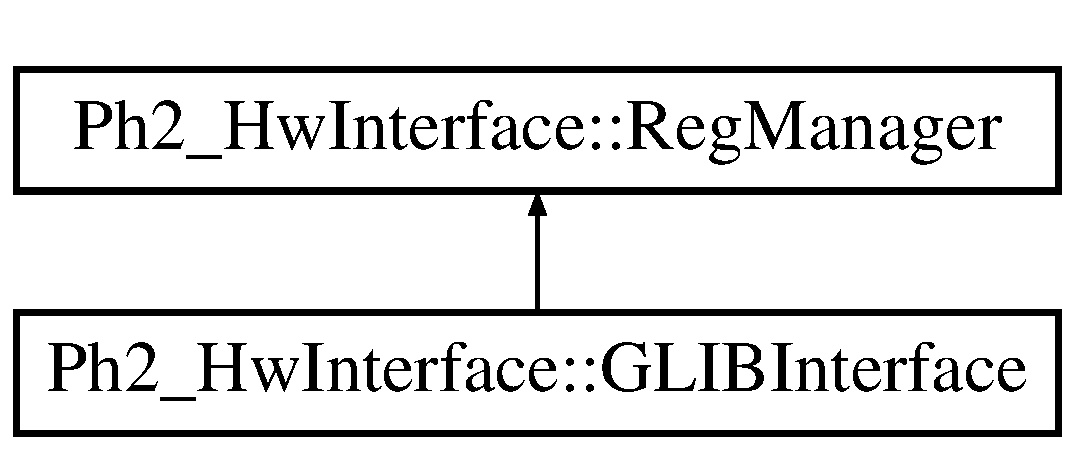
\includegraphics[height=2.000000cm]{class_ph2___hw_interface_1_1_g_l_i_b_interface}
\end{center}
\end{figure}
\subsection*{Public Member Functions}
\begin{DoxyCompactItemize}
\item 
\hypertarget{class_ph2___hw_interface_1_1_g_l_i_b_interface_a6c11567e50b46ee41894ef4b55aa6ef9}{{\bfseries G\-L\-I\-B\-Interface} (const char $\ast$pu\-Hal\-Config\-File\-Name, const char $\ast$p\-Board\-Id)}\label{class_ph2___hw_interface_1_1_g_l_i_b_interface_a6c11567e50b46ee41894ef4b55aa6ef9}

\item 
\hypertarget{class_ph2___hw_interface_1_1_g_l_i_b_interface_a184c9b6bff4282e42218f66115627c91}{void {\bfseries Configure\-G\-L\-I\-B} ()}\label{class_ph2___hw_interface_1_1_g_l_i_b_interface_a184c9b6bff4282e42218f66115627c91}

\item 
\hypertarget{class_ph2___hw_interface_1_1_g_l_i_b_interface_a302bb9d57200f2da4889d5eb503777b8}{void {\bfseries Start} ()}\label{class_ph2___hw_interface_1_1_g_l_i_b_interface_a302bb9d57200f2da4889d5eb503777b8}

\item 
\hypertarget{class_ph2___hw_interface_1_1_g_l_i_b_interface_a9e17e9e892909e4e21f0066264ff852f}{void {\bfseries Stop} (uint32\-\_\-t p\-Nth\-Acq)}\label{class_ph2___hw_interface_1_1_g_l_i_b_interface_a9e17e9e892909e4e21f0066264ff852f}

\item 
\hypertarget{class_ph2___hw_interface_1_1_g_l_i_b_interface_a10d686f98e2978d93647aaf250404508}{void {\bfseries Pause} ()}\label{class_ph2___hw_interface_1_1_g_l_i_b_interface_a10d686f98e2978d93647aaf250404508}

\item 
\hypertarget{class_ph2___hw_interface_1_1_g_l_i_b_interface_a6a9df619d8d0c3961f9ae635cc5389c8}{void {\bfseries Unpause} ()}\label{class_ph2___hw_interface_1_1_g_l_i_b_interface_a6a9df619d8d0c3961f9ae635cc5389c8}

\item 
\hypertarget{class_ph2___hw_interface_1_1_g_l_i_b_interface_afdd87a6f34631f8d9cfba4409b6be979}{void {\bfseries Read\-D\-A\-Q} (uint32\-\_\-t p\-Nth\-Acq, bool p\-Break\-Trigger)}\label{class_ph2___hw_interface_1_1_g_l_i_b_interface_afdd87a6f34631f8d9cfba4409b6be979}

\item 
\hypertarget{class_ph2___hw_interface_1_1_g_l_i_b_interface_a8d97c10041d2376b17aa460b09ba02f6}{void {\bfseries S\-R\-A\-Mfor\-D\-A\-Q} (uint32\-\_\-t p\-Nth\-Acq)}\label{class_ph2___hw_interface_1_1_g_l_i_b_interface_a8d97c10041d2376b17aa460b09ba02f6}

\end{DoxyCompactItemize}
\subsection*{Static Public Attributes}
\begin{DoxyCompactItemize}
\item 
\hypertarget{class_ph2___hw_interface_1_1_g_l_i_b_interface_a85f9c804b41b8eb7b4d81f7307b5bc4a}{static unsigned int {\bfseries N\-Be} = 0}\label{class_ph2___hw_interface_1_1_g_l_i_b_interface_a85f9c804b41b8eb7b4d81f7307b5bc4a}

\item 
\hypertarget{class_ph2___hw_interface_1_1_g_l_i_b_interface_a7e34fbc5d0399cb77d070c8062e104f9}{static unsigned int {\bfseries f\-Packet\-Size} = E\-V\-E\-N\-T\-\_\-\-S\-I\-Z\-E\-\_\-32}\label{class_ph2___hw_interface_1_1_g_l_i_b_interface_a7e34fbc5d0399cb77d070c8062e104f9}

\end{DoxyCompactItemize}
\subsection*{Additional Inherited Members}


The documentation for this class was generated from the following files\-:\begin{DoxyCompactItemize}
\item 
G\-L\-I\-B\-Interface.\-h\item 
G\-L\-I\-B\-Interface.\-cc\end{DoxyCompactItemize}

\hypertarget{class_ph2___hw_interface_1_1_reg_manager}{\section{Ph2\-\_\-\-Hw\-Interface\-:\-:Reg\-Manager Class Reference}
\label{class_ph2___hw_interface_1_1_reg_manager}\index{Ph2\-\_\-\-Hw\-Interface\-::\-Reg\-Manager@{Ph2\-\_\-\-Hw\-Interface\-::\-Reg\-Manager}}
}


Permit connection to given boards and r/w given registers.  




{\ttfamily \#include $<$Reg\-Manager.\-h$>$}

Inheritance diagram for Ph2\-\_\-\-Hw\-Interface\-:\-:Reg\-Manager\-:\begin{figure}[H]
\begin{center}
\leavevmode
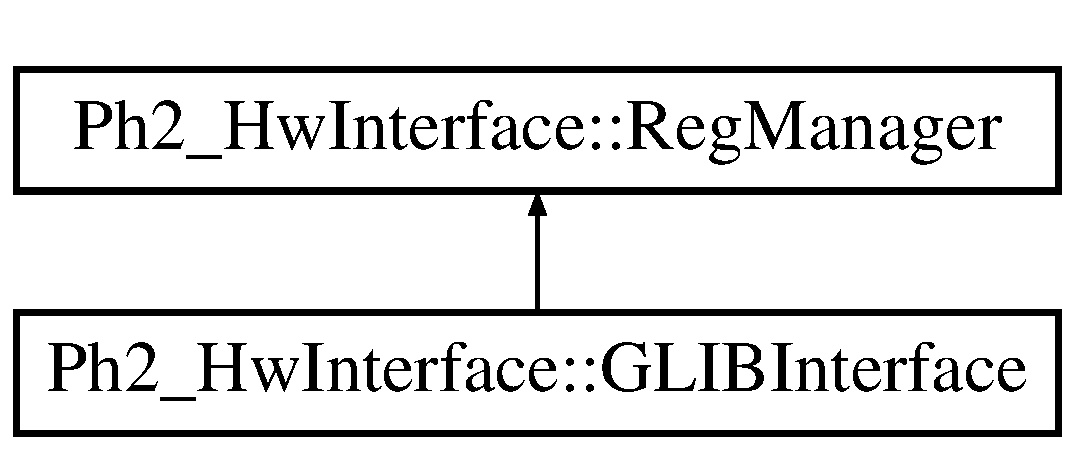
\includegraphics[height=2.000000cm]{class_ph2___hw_interface_1_1_reg_manager}
\end{center}
\end{figure}
\subsection*{Public Member Functions}
\begin{DoxyCompactItemize}
\item 
\hyperlink{class_ph2___hw_interface_1_1_reg_manager_a938f6b582b1fffcb478f35fd9d81954f}{Reg\-Manager} (const char $\ast$pu\-Hal\-Config\-File\-Name)
\begin{DoxyCompactList}\small\item\em Constructor of the \hyperlink{class_ph2___hw_interface_1_1_reg_manager}{Reg\-Manager} class. \end{DoxyCompactList}\item 
virtual \hyperlink{class_ph2___hw_interface_1_1_reg_manager_a5d650c4e6467153f98f999abbbfc354c}{$\sim$\-Reg\-Manager} ()
\begin{DoxyCompactList}\small\item\em Destructor of the \hyperlink{class_ph2___hw_interface_1_1_reg_manager}{Reg\-Manager} class. \end{DoxyCompactList}\end{DoxyCompactItemize}
\subsection*{Protected Member Functions}
\begin{DoxyCompactItemize}
\item 
virtual bool \hyperlink{class_ph2___hw_interface_1_1_reg_manager_a31174516fef6706c88c3f59dd93e4fdf}{Write\-Reg} (const std\-::string \&p\-Reg\-Node, const uint32\-\_\-t \&p\-Val)
\begin{DoxyCompactList}\small\item\em Write a register. \end{DoxyCompactList}\item 
virtual bool \hyperlink{class_ph2___hw_interface_1_1_reg_manager_a888f5cccb05daa28896cf622abfdcbd6}{Write\-Block\-Reg} (const std\-::string \&p\-Reg\-Node, const std\-::vector$<$ uint32\-\_\-t $>$ \&p\-Values)
\begin{DoxyCompactList}\small\item\em Write a block of values in a register. \end{DoxyCompactList}\item 
virtual uhal\-::\-Val\-Word$<$ uint32\-\_\-t $>$ \hyperlink{class_ph2___hw_interface_1_1_reg_manager_a077e0a18592206365150680213345112}{Read\-Reg} (const std\-::string \&p\-Reg\-Node)
\begin{DoxyCompactList}\small\item\em Read a value in a register. \end{DoxyCompactList}\item 
virtual uhal\-::\-Val\-Vector$<$ uint32\-\_\-t $>$ \hyperlink{class_ph2___hw_interface_1_1_reg_manager_a6481c211d27badc409ff0e7af20575e4}{Read\-Block\-Reg} (const std\-::string \&p\-Reg\-Node, const uint32\-\_\-t \&p\-Blocksize)
\begin{DoxyCompactList}\small\item\em Read a block of values in a register. \end{DoxyCompactList}\item 
virtual void \hyperlink{class_ph2___hw_interface_1_1_reg_manager_a20c502bcad5115c6ae16d4d356b72f0c}{Choose\-Board} (uint8\-\_\-t p\-Board\-Id)
\begin{DoxyCompactList}\small\item\em Choose the board we want to talk with. \end{DoxyCompactList}\end{DoxyCompactItemize}
\subsection*{Protected Attributes}
\begin{DoxyCompactItemize}
\item 
uhal\-::\-Hw\-Interface $\ast$ \hyperlink{class_ph2___hw_interface_1_1_reg_manager_a0d4908ec834a3a0b7d8139872fd0a4a0}{f\-Board}
\item 
const char $\ast$ \hyperlink{class_ph2___hw_interface_1_1_reg_manager_aaaa29ca65c283acc645132c7bef0f24f}{f\-U\-Hal\-Config\-File\-Name}
\item 
std\-::map$<$ uint8\-\_\-t, \\*
uhal\-::\-Hw\-Interface $\ast$ $>$ \hyperlink{class_ph2___hw_interface_1_1_reg_manager_a9c34ffe467a572796c05036533bb6d39}{f\-Board\-Map}
\end{DoxyCompactItemize}


\subsection{Detailed Description}
Permit connection to given boards and r/w given registers. 

\subsection{Constructor \& Destructor Documentation}
\hypertarget{class_ph2___hw_interface_1_1_reg_manager_a938f6b582b1fffcb478f35fd9d81954f}{\index{Ph2\-\_\-\-Hw\-Interface\-::\-Reg\-Manager@{Ph2\-\_\-\-Hw\-Interface\-::\-Reg\-Manager}!Reg\-Manager@{Reg\-Manager}}
\index{Reg\-Manager@{Reg\-Manager}!Ph2_HwInterface::RegManager@{Ph2\-\_\-\-Hw\-Interface\-::\-Reg\-Manager}}
\subsubsection[{Reg\-Manager}]{\setlength{\rightskip}{0pt plus 5cm}Ph2\-\_\-\-Hw\-Interface\-::\-Reg\-Manager\-::\-Reg\-Manager (
\begin{DoxyParamCaption}
\item[{const char $\ast$}]{pu\-Hal\-Config\-File\-Name}
\end{DoxyParamCaption}
)}}\label{class_ph2___hw_interface_1_1_reg_manager_a938f6b582b1fffcb478f35fd9d81954f}


Constructor of the \hyperlink{class_ph2___hw_interface_1_1_reg_manager}{Reg\-Manager} class. 


\begin{DoxyParams}{Parameters}
{\em pu\-Hal\-Config\-File\-Name} & \-: path of the u\-Hal Config File \\
\hline
\end{DoxyParams}
\hypertarget{class_ph2___hw_interface_1_1_reg_manager_a5d650c4e6467153f98f999abbbfc354c}{\index{Ph2\-\_\-\-Hw\-Interface\-::\-Reg\-Manager@{Ph2\-\_\-\-Hw\-Interface\-::\-Reg\-Manager}!$\sim$\-Reg\-Manager@{$\sim$\-Reg\-Manager}}
\index{$\sim$\-Reg\-Manager@{$\sim$\-Reg\-Manager}!Ph2_HwInterface::RegManager@{Ph2\-\_\-\-Hw\-Interface\-::\-Reg\-Manager}}
\subsubsection[{$\sim$\-Reg\-Manager}]{\setlength{\rightskip}{0pt plus 5cm}Ph2\-\_\-\-Hw\-Interface\-::\-Reg\-Manager\-::$\sim$\-Reg\-Manager (
\begin{DoxyParamCaption}
{}
\end{DoxyParamCaption}
)\hspace{0.3cm}{\ttfamily [virtual]}}}\label{class_ph2___hw_interface_1_1_reg_manager_a5d650c4e6467153f98f999abbbfc354c}


Destructor of the \hyperlink{class_ph2___hw_interface_1_1_reg_manager}{Reg\-Manager} class. 



\subsection{Member Function Documentation}
\hypertarget{class_ph2___hw_interface_1_1_reg_manager_a20c502bcad5115c6ae16d4d356b72f0c}{\index{Ph2\-\_\-\-Hw\-Interface\-::\-Reg\-Manager@{Ph2\-\_\-\-Hw\-Interface\-::\-Reg\-Manager}!Choose\-Board@{Choose\-Board}}
\index{Choose\-Board@{Choose\-Board}!Ph2_HwInterface::RegManager@{Ph2\-\_\-\-Hw\-Interface\-::\-Reg\-Manager}}
\subsubsection[{Choose\-Board}]{\setlength{\rightskip}{0pt plus 5cm}void Ph2\-\_\-\-Hw\-Interface\-::\-Reg\-Manager\-::\-Choose\-Board (
\begin{DoxyParamCaption}
\item[{uint8\-\_\-t}]{p\-Board\-Id}
\end{DoxyParamCaption}
)\hspace{0.3cm}{\ttfamily [protected]}, {\ttfamily [virtual]}}}\label{class_ph2___hw_interface_1_1_reg_manager_a20c502bcad5115c6ae16d4d356b72f0c}


Choose the board we want to talk with. 


\begin{DoxyParams}{Parameters}
{\em p\-Board\-Id} & \-: Id of the Board to connect to \\
\hline
\end{DoxyParams}
\hypertarget{class_ph2___hw_interface_1_1_reg_manager_a6481c211d27badc409ff0e7af20575e4}{\index{Ph2\-\_\-\-Hw\-Interface\-::\-Reg\-Manager@{Ph2\-\_\-\-Hw\-Interface\-::\-Reg\-Manager}!Read\-Block\-Reg@{Read\-Block\-Reg}}
\index{Read\-Block\-Reg@{Read\-Block\-Reg}!Ph2_HwInterface::RegManager@{Ph2\-\_\-\-Hw\-Interface\-::\-Reg\-Manager}}
\subsubsection[{Read\-Block\-Reg}]{\setlength{\rightskip}{0pt plus 5cm}uhal\-::\-Val\-Vector$<$ uint32\-\_\-t $>$ Ph2\-\_\-\-Hw\-Interface\-::\-Reg\-Manager\-::\-Read\-Block\-Reg (
\begin{DoxyParamCaption}
\item[{const std\-::string \&}]{p\-Reg\-Node, }
\item[{const uint32\-\_\-t \&}]{p\-Blocksize}
\end{DoxyParamCaption}
)\hspace{0.3cm}{\ttfamily [protected]}, {\ttfamily [virtual]}}}\label{class_ph2___hw_interface_1_1_reg_manager_a6481c211d27badc409ff0e7af20575e4}


Read a block of values in a register. 


\begin{DoxyParams}{Parameters}
{\em p\-Reg\-Node} & \-: Node of the register to read \\
\hline
{\em p\-Blocksize} & \-: Size of the block to read \\
\hline
\end{DoxyParams}
\begin{DoxyReturn}{Returns}
Val\-Vector block values of the register 
\end{DoxyReturn}
\hypertarget{class_ph2___hw_interface_1_1_reg_manager_a077e0a18592206365150680213345112}{\index{Ph2\-\_\-\-Hw\-Interface\-::\-Reg\-Manager@{Ph2\-\_\-\-Hw\-Interface\-::\-Reg\-Manager}!Read\-Reg@{Read\-Reg}}
\index{Read\-Reg@{Read\-Reg}!Ph2_HwInterface::RegManager@{Ph2\-\_\-\-Hw\-Interface\-::\-Reg\-Manager}}
\subsubsection[{Read\-Reg}]{\setlength{\rightskip}{0pt plus 5cm}uhal\-::\-Val\-Word$<$ uint32\-\_\-t $>$ Ph2\-\_\-\-Hw\-Interface\-::\-Reg\-Manager\-::\-Read\-Reg (
\begin{DoxyParamCaption}
\item[{const std\-::string \&}]{p\-Reg\-Node}
\end{DoxyParamCaption}
)\hspace{0.3cm}{\ttfamily [protected]}, {\ttfamily [virtual]}}}\label{class_ph2___hw_interface_1_1_reg_manager_a077e0a18592206365150680213345112}


Read a value in a register. 


\begin{DoxyParams}{Parameters}
{\em p\-Reg\-Node} & \-: Node of the register to read \\
\hline
\end{DoxyParams}
\begin{DoxyReturn}{Returns}
Val\-Word value of the register 
\end{DoxyReturn}
\hypertarget{class_ph2___hw_interface_1_1_reg_manager_a888f5cccb05daa28896cf622abfdcbd6}{\index{Ph2\-\_\-\-Hw\-Interface\-::\-Reg\-Manager@{Ph2\-\_\-\-Hw\-Interface\-::\-Reg\-Manager}!Write\-Block\-Reg@{Write\-Block\-Reg}}
\index{Write\-Block\-Reg@{Write\-Block\-Reg}!Ph2_HwInterface::RegManager@{Ph2\-\_\-\-Hw\-Interface\-::\-Reg\-Manager}}
\subsubsection[{Write\-Block\-Reg}]{\setlength{\rightskip}{0pt plus 5cm}bool Ph2\-\_\-\-Hw\-Interface\-::\-Reg\-Manager\-::\-Write\-Block\-Reg (
\begin{DoxyParamCaption}
\item[{const std\-::string \&}]{p\-Reg\-Node, }
\item[{const std\-::vector$<$ uint32\-\_\-t $>$ \&}]{p\-Values}
\end{DoxyParamCaption}
)\hspace{0.3cm}{\ttfamily [protected]}, {\ttfamily [virtual]}}}\label{class_ph2___hw_interface_1_1_reg_manager_a888f5cccb05daa28896cf622abfdcbd6}


Write a block of values in a register. 


\begin{DoxyParams}{Parameters}
{\em p\-Reg\-Node} & \-: Node of the register to write \\
\hline
{\em p\-Values} & \-: Block of values to write \\
\hline
\end{DoxyParams}
\begin{DoxyReturn}{Returns}
boolean confirming the writing 
\end{DoxyReturn}
\hypertarget{class_ph2___hw_interface_1_1_reg_manager_a31174516fef6706c88c3f59dd93e4fdf}{\index{Ph2\-\_\-\-Hw\-Interface\-::\-Reg\-Manager@{Ph2\-\_\-\-Hw\-Interface\-::\-Reg\-Manager}!Write\-Reg@{Write\-Reg}}
\index{Write\-Reg@{Write\-Reg}!Ph2_HwInterface::RegManager@{Ph2\-\_\-\-Hw\-Interface\-::\-Reg\-Manager}}
\subsubsection[{Write\-Reg}]{\setlength{\rightskip}{0pt plus 5cm}bool Ph2\-\_\-\-Hw\-Interface\-::\-Reg\-Manager\-::\-Write\-Reg (
\begin{DoxyParamCaption}
\item[{const std\-::string \&}]{p\-Reg\-Node, }
\item[{const uint32\-\_\-t \&}]{p\-Val}
\end{DoxyParamCaption}
)\hspace{0.3cm}{\ttfamily [protected]}, {\ttfamily [virtual]}}}\label{class_ph2___hw_interface_1_1_reg_manager_a31174516fef6706c88c3f59dd93e4fdf}


Write a register. 


\begin{DoxyParams}{Parameters}
{\em p\-Reg\-Node} & \-: Node of the register to write \\
\hline
{\em p\-Val} & \-: Value to write \\
\hline
\end{DoxyParams}
\begin{DoxyReturn}{Returns}
boolean confirming the writing 
\end{DoxyReturn}


\subsection{Field Documentation}
\hypertarget{class_ph2___hw_interface_1_1_reg_manager_a0d4908ec834a3a0b7d8139872fd0a4a0}{\index{Ph2\-\_\-\-Hw\-Interface\-::\-Reg\-Manager@{Ph2\-\_\-\-Hw\-Interface\-::\-Reg\-Manager}!f\-Board@{f\-Board}}
\index{f\-Board@{f\-Board}!Ph2_HwInterface::RegManager@{Ph2\-\_\-\-Hw\-Interface\-::\-Reg\-Manager}}
\subsubsection[{f\-Board}]{\setlength{\rightskip}{0pt plus 5cm}uhal\-::\-Hw\-Interface$\ast$ Ph2\-\_\-\-Hw\-Interface\-::\-Reg\-Manager\-::f\-Board\hspace{0.3cm}{\ttfamily [protected]}}}\label{class_ph2___hw_interface_1_1_reg_manager_a0d4908ec834a3a0b7d8139872fd0a4a0}
Board in use \hypertarget{class_ph2___hw_interface_1_1_reg_manager_a9c34ffe467a572796c05036533bb6d39}{\index{Ph2\-\_\-\-Hw\-Interface\-::\-Reg\-Manager@{Ph2\-\_\-\-Hw\-Interface\-::\-Reg\-Manager}!f\-Board\-Map@{f\-Board\-Map}}
\index{f\-Board\-Map@{f\-Board\-Map}!Ph2_HwInterface::RegManager@{Ph2\-\_\-\-Hw\-Interface\-::\-Reg\-Manager}}
\subsubsection[{f\-Board\-Map}]{\setlength{\rightskip}{0pt plus 5cm}std\-::map$<$uint8\-\_\-t,uhal\-::\-Hw\-Interface$\ast$$>$ Ph2\-\_\-\-Hw\-Interface\-::\-Reg\-Manager\-::f\-Board\-Map\hspace{0.3cm}{\ttfamily [protected]}}}\label{class_ph2___hw_interface_1_1_reg_manager_a9c34ffe467a572796c05036533bb6d39}
Board Map with all known boards \hypertarget{class_ph2___hw_interface_1_1_reg_manager_aaaa29ca65c283acc645132c7bef0f24f}{\index{Ph2\-\_\-\-Hw\-Interface\-::\-Reg\-Manager@{Ph2\-\_\-\-Hw\-Interface\-::\-Reg\-Manager}!f\-U\-Hal\-Config\-File\-Name@{f\-U\-Hal\-Config\-File\-Name}}
\index{f\-U\-Hal\-Config\-File\-Name@{f\-U\-Hal\-Config\-File\-Name}!Ph2_HwInterface::RegManager@{Ph2\-\_\-\-Hw\-Interface\-::\-Reg\-Manager}}
\subsubsection[{f\-U\-Hal\-Config\-File\-Name}]{\setlength{\rightskip}{0pt plus 5cm}const char$\ast$ Ph2\-\_\-\-Hw\-Interface\-::\-Reg\-Manager\-::f\-U\-Hal\-Config\-File\-Name\hspace{0.3cm}{\ttfamily [protected]}}}\label{class_ph2___hw_interface_1_1_reg_manager_aaaa29ca65c283acc645132c7bef0f24f}
path of the u\-Hal Config File 

The documentation for this class was generated from the following files\-:\begin{DoxyCompactItemize}
\item 
H\-W\-Interface/\hyperlink{_reg_manager_8h}{Reg\-Manager.\-h}\item 
H\-W\-Interface/\hyperlink{_reg_manager_8cc}{Reg\-Manager.\-cc}\end{DoxyCompactItemize}

%--- End generated contents ---

% Index
\newpage
\phantomsection
\addcontentsline{toc}{part}{Index}
\printindex

\end{document}
